\def\year{2019}\relax
%File: formatting-instruction.tex
\documentclass[letterpaper]{article} %DO NOT CHANGE THIS
\usepackage{aaai19}  %Required
\usepackage{times}  %Required
\usepackage{helvet}  %Required
\usepackage{courier}  %Required
\usepackage{url}  %Required
\usepackage{graphicx}  %Required
\usepackage{fixltx2e} %Required
\frenchspacing  %Required
\setlength{\pdfpagewidth}{8.5in}  %Required
\setlength{\pdfpageheight}{11in}  %Required
%PDF Info Is Required:
  \pdfinfo{
/Title (Title and Image Based Classification of Magic: The Gathering Cards)
/Author (Derick Anderson, Zachary Reiter)}
\setcounter{secnumdepth}{0}
\nocopyright
\graphicspath{ {./imgs/} }
 \begin{document}
% The file aaai.sty is the style file for AAAI Press
% proceedings, working notes, and technical reports.
%
\title{Title and Image Based Classification of Magic: The Gathering Cards}
\author{Derick Anderson \ and Zachary Reiter\\
  anderson.derick.w@gmail.com\\
  reiter.z@husky.neu.edu
}
\maketitle
\begin{abstract}
magic!
\end{abstract}



\section{Background}

is a card game

\section{Related Work}

Image classification is a popular application of neural networks,
and there are several general solutions that already exist. We wanted to start with an
image classification model and tune the implementation and training parameters
to see if the current state of the art models were sufficient for this task.
We looked at InceptionV3 which looked promising, but we decided against it
because we felt the resources it demanded would be beyond what we were able to
obtain \cite{SzegedyChristian2015RtIA}. We looked into smaller models that used fewer
parameters and so would require less memory for storing weights. We found the
DenseNet architecture, which won the best Paper Award at CVPR in
2017 \cite{huang2017densely}. The main paradigm is that each layer is connected to each
other layer in a feed forward fashion within a Dense block which consists of
convolutions and pooling operations \cite{huang2017densely}.

\begin{figure}
  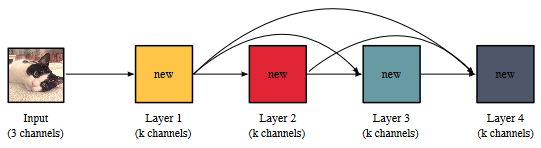
\includegraphics[width=.5\textwidth]{densenet}
  \caption{Illustration of the DenseNet architecture, from \cite{PleissGeoff2017MIoD}}
\end{figure}

According to their experiments, it yields competitive accuracy while using less
than half of the parameters used by other architectures like ResNet. It looked
promising, but we wanted to find evidence that it was useful practically as
well. In 2018 Rajaraman, Antani, Poostchi, Silamut, Hossain, Maude, Jaeger,
and Thoma used the DenseNet-121 implementation in their research using CNN’s
to detect malaria parasites in blood smears \cite{RajaramanSivaramakrishnan2018Pcnn}.
We located an MIT
licensed implementation of DenseNet-121 at
https://github.com/flyyufelix/DenseNet-Keras and decided this would be our
default model for image classification [cite web source?]. It included a set of
weights pre-trained on the ImageNet data set as well, meaning we could compare
fine tuning this model on our data against training the model on our data from
scratch. The model implementation and our code uses Keras as a high level
interface for working with Tensorflow models \cite{chollet2015keras}.

\section{Project Description}

\subsection{Title-based Classification}

The architecture used for title classification
was a character-level LSTM with self-attention.
The LSTM \cite{Hochreiter1997LongSM} is a recurrent neural network architecture
that is frequently and effectively \cite{Schmidhuber2015DeepLI}
used to process text data.
Because it is such a well known architecture
we will not reproduce here its fundamental structure.
We will discuss the extensions to the basic LSTM that were used.

The LSTM was character-level,
which means that timesteps were taken to be each character in the title.
The characters were embedded in vector space
before being passed into the LSTM as input.
The character embeddings were learned from scratch
in a fully end-to-end manner.

Attention is a mechanism for combining a sequence of values into a single value
with learnable parameters.
We use the multi-headed self-attention mechanism from \cite{Lin2017ASS}
over the outputs of the LSTM and before our output layer.
It was shown to enhance peformance on some classification tasks
(as compared to passing the final state of the LSTM to the output layer)
and as a bonus permits attractive visualizations
of which portions of the input sequence contribute to the output.

The optimizer used was Adam \cite{Kingma2014AdamAM}
with norm-based gradient clipping \cite{Pascanu2012UnderstandingTE}.

\begin{figure}
  \centering
  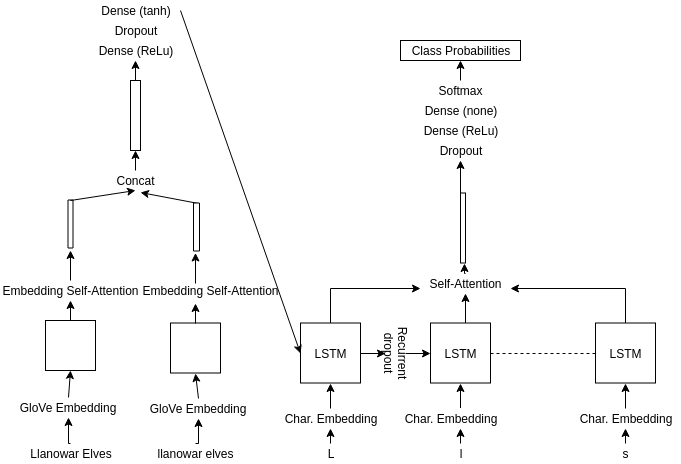
\includegraphics[width=.45\textwidth]{text-architecture}
  \caption{Title-based model architecture}
\end{figure}

\subsubsection{Word Embeddings}

In one variation of the model
the initial state of the LSTM
is created from the embeddings of words in the title.
We used pre-trained GloVe \cite{Pennington2014GloveGV} embeddings,
specifically the 840B token Common Crawl set
available for download from the Stanford NLP group's website
\footnote{https://nlp.stanford.edu/projects/glove/}.
Using pre-trained word embeddings
was motivated by the need for lexical knowledge in classifying titles.
On an intuitive level many titles for creatures
contain words that describe people/animals etc,
and the other categories likewise often have informative English words.

We combine sequences of word embeddings with a small self-attention layer.
That set of word embeddings is case-sensitive,
so we concatenate the attended result of embedding
the word-level tokens of the title as-is
and the tokens converted to lower case.
Card titles are title cased,
so it was helpful to get the embedding of common nouns in the title
in their lower cased form.
For example,
``Merfolk Looter''
has a more informative (and more likely to be in the vocabulary)
embedding for ``looter'' than for ``Looter''.

The GloVe data we downloaded has a vocabulary of over 2 million ``words'',
but we use only the embeddings representing the most common 200,000.
On a practical computational level,
it is difficult to incorporate such large matrices into a model.
On another level,
it was observed that many MtG-specific proper nouns are in the full vocabulary.
Insofar as Magic: The Gathering is a popular topic online and the word embeddings
are based on web crawl data that only makes sense.
However,
it was considered not quite in the spirit of the task
for MtG-specific proper nouns to be in-vocabulary.
A selection of the most common MtG-specific proper nouns were investigated
and found to be below the 200,000th most common mark.
More general myth-related or fantastical terms (e.g. ``elf'', ``merfolk'')
largely remained in the vocabulary.
Out-of-vocabulary terms were assigned a randomly initialized embedding.

\subsubsection{Regularization}

Given the small size of the training data thorough regularization was a must.
The methods of regularization used were
L2 regularization on the weights of the dense layers,
dropout between dense layers,
recurrent dropout (as described in \cite{Gal2016ATG}) in the LSTM,
and the penalty described in \cite{Lin2017ASS} for the self-attention layer.
Card titles consisted only of ASCII characters;
the distribution of characters was not particularly sparse
and so no regularization directly on the character embeddings
was thought to be necessary.
No regularization was needed on the word embeddings since they were not trained.

\subsection{Image-based Classification}

We used a DenseNet-121 model for image classification and experimented with
tuning the training parameters and optimizers to achieve the best result.
DenseNet-121 uses the output of each dense block layer as an input to each
subsequent dense block [DenseNet, 2]. This is different from traditional
convolutional feed-forward networks. Let’s an image x\textsubscript{0} is passed through a
convolutional network of L layers which each have a transformation H\textsubscript{l}, where l
is the layer number [DenseNet, 2]. Traditional networks have the formula
x\textsubscript{l} = H\textsubscript{l}(x\textsubscript{l}-1), but DenseNet-121 looks more like:

\begin{center}
  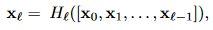
\includegraphics[width=.3\textwidth]{densenet-formula}
\end{center}

We wanted to see how well suited this model was for the task of classifying Magic cards,
but we experimented with several optimization and training configurations,
outlined below.

\section{Experiments}


\subsection{Title-based Classification}

\begin{table}
  \centering
  \caption{Hyperparameters of the final title-based model}
  \begin{tabular}{r | c | c}
    Hyperparameter & Value (small) & (large) \\
    \hline
    LSTM Size & 256 & 512 \\
    Character embedding size & 64 & 128 \\
    Attention, number of heads ($r$) & 3 & 3\\
    Attention, attention size ($d_a$) & 64 & 128\\
    Dropout rate & 0.5 & 0.5 \\
    L2 regularization coef. & 1e-4 & 1e-4 \\
    Attention regularization coef. & 4e-4 & 4e-4 \\
    Gradient clipping threshold & 5.0 & 5.0 \\
  \end{tabular}
\end{table}

Unfortunately,
due to time constraints,
there was not the opportunity for an organized hyperparameter search.
Instead,
reasonable values were chosen from experience and the literature
and only a little local search performed.
Interestingly the smaller configuration outperformed the larger configuration
on the reported results.
That can be attributed partially to noise in the results,
and also to the danger of overfitting on the small data.
Either way,
the smaller model configuration is therefore used for all following analyses.
It is clear from the results that the lexical knowledge supplied by word vectors
is very helpful to the model.

\begin{table}
  \centering
  \caption{Test scores on all data for different model configurations}
  \begin{tabular}{r | c | c}
    Model configuration & Accuracy & Macro-averaged F1 \\
    \hline
    Small & 80.6\% &  .642 \\
    Larger & 79.2\% & .638 \\
    Character-only & 71.3\% & .523 \\
    Largest class & 55.6\% & .179 \\
  \end{tabular}
\end{table}

It is interesting to compare the speed with which the character-only
and the full model learned.
The full model reached its maximum accuracy on the validation set quite quickly,
whereas it took the character-only model 25 epochs to reach its maximum.
That the character model can productively learn for 25 epochs
suggests that either the character information is redundant
in the presence of word embeddings
or the full model isn't learning optimally.
Looking at the distribution of attention intensity
also suggests that the full model doesn't pay a lot of attention to the characters.
The attention heads for the character model focus at a few different points,
the embedding model's attention is much more diffuse
(except for at the first position,
where I speculate the first head reports
the information gained from the initial state).

\begin{figure}
  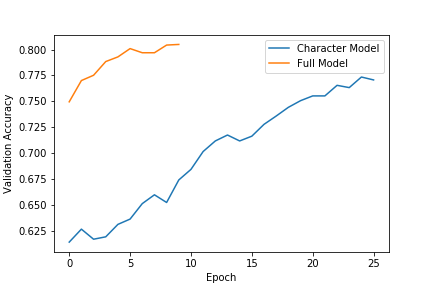
\includegraphics[width=.5\textwidth]{training-speed-comparison}
  \caption{Validation accuracy over time for character-only model vs. full model}
\end{figure}

\begin{figure}
  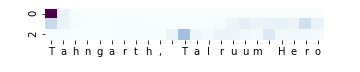
\includegraphics[width=.5\textwidth]{tahngarth-attention-wv}
  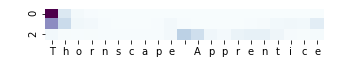
\includegraphics[width=.5\textwidth]{thornscape-attention-wv}
  \caption{Attention intensity for full model}
\end{figure}

\begin{figure}
  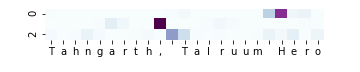
\includegraphics[width=.5\textwidth]{tahngarth-attention-char}
  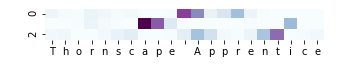
\includegraphics[width=.5\textwidth]{thornscape-attention-char}
  \caption{Attention intensity for character-only model}
\end{figure}

\begin{table}
  \centering
  \caption{Macro-averaged F1 by training and testing dataset}
  \begin{tabular}{r | c | c | c}
    & \multicolumn{3}{c}{Test dataset}\\
    \cline{2-4}
    Train dataset & all & modern & legacy \\
    \hline
    all    & .642 & .643 & .645 \\
    modern & .602 & .643 & .573 \\
    legacy & .622 & .597 & .639 \\
  \end{tabular}
\end{table}

\begin{table}
  \centering
  \caption{Accuracy by training and testing dataset}
  \begin{tabular}{r | c | c | c}
    & \multicolumn{3}{c}{Test dataset}\\
    \cline{2-4}
    Train dataset & all & modern & legacy \\
    \hline
    all    & 80.6\% & 81.2\% & 80.1\% \\
    modern & 76.0\% & 78.3\% & 74.1\% \\
    legacy & 76.4\% & 75.1\% & 77.0\% \\
  \end{tabular}
\end{table}

As predicted from the beginning,
training on one of the genres of data
and testing on the other genre leads to reduced performance.
It appears that training on the legacy cards
transfers more easily to the modern cards
than vice-versa,
to the tune of a few points of accuracy.

\begin{figure}
  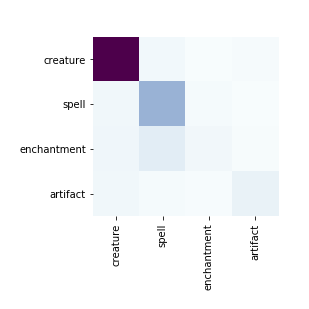
\includegraphics[width=.5\textwidth]{text-confusion-matrix}
  \caption{Confusion matrix: predicted is on the x axis}
\end{figure}

The confusion matrix matches our intuitions fairly well.
The two classes with the largest confusion are spell and enchantment,
which while distinct in the game mechanics
are certainly the semantically closest in an abstract sense.

\subsection{Image-based Classification}

We focused on the following variables to alter in order to affect performance:
number of epochs, learning rate reduction, optimizer type
(Adam or Stochastic Gradient Descent), optimizer configuration (decay rate,
descent momentum), early stopping, and image scaling.
We first got a baseline performance for each model using the following
configurations: 20 epochs, no learning rate reduction, Adam optimizer,
no decay rate, no early stopping, image size 50x50. The performance of this can
be see in Figure ~\ref{fig:baseline}

\begin{figure}
  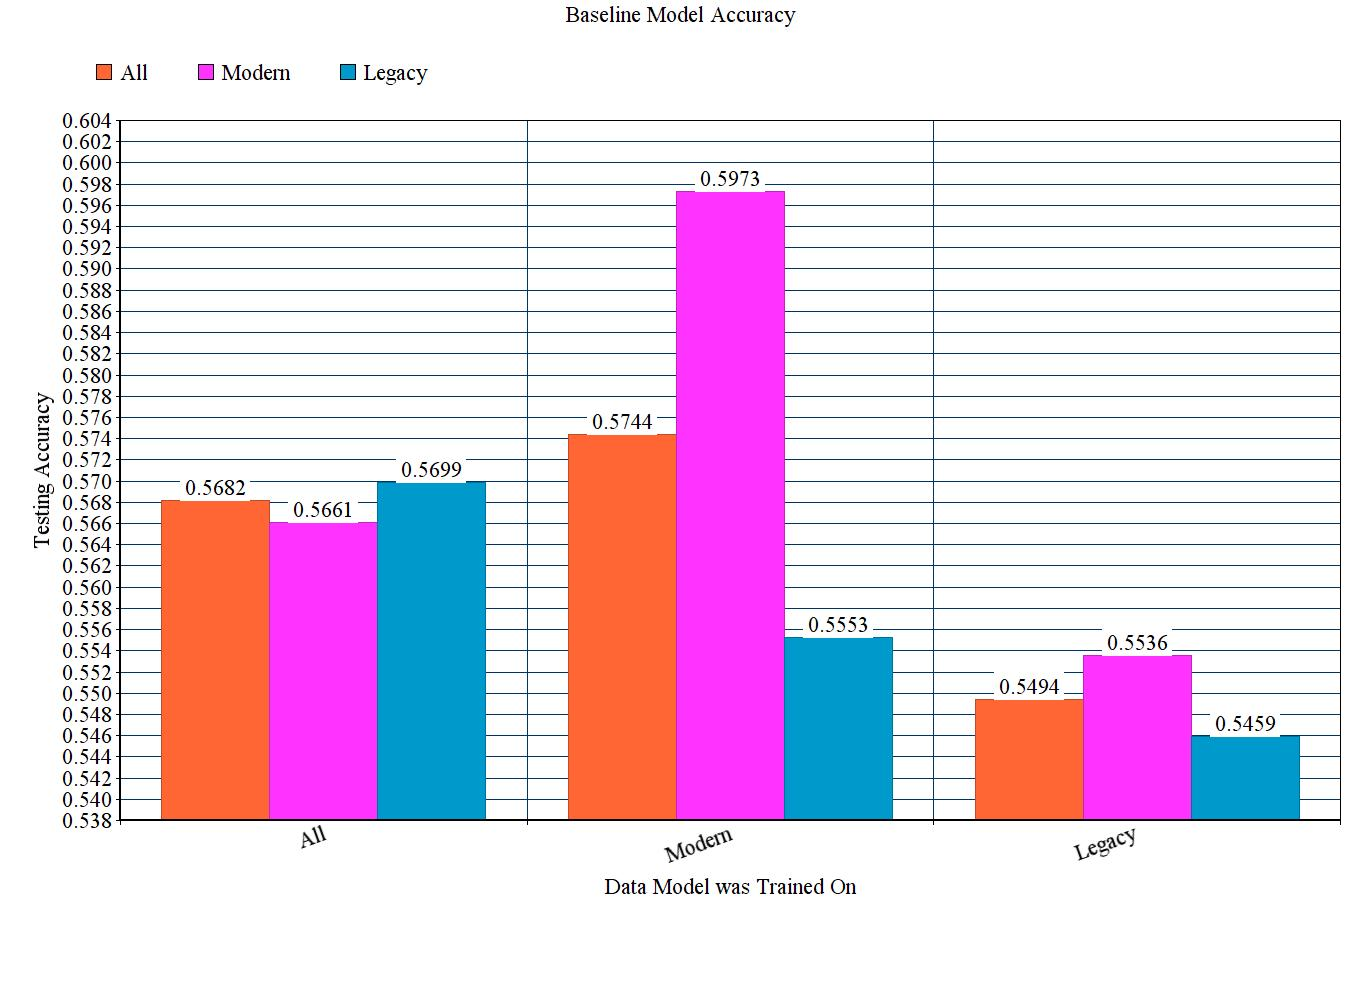
\includegraphics[width=.5\textwidth]{baseline-accuracy}
  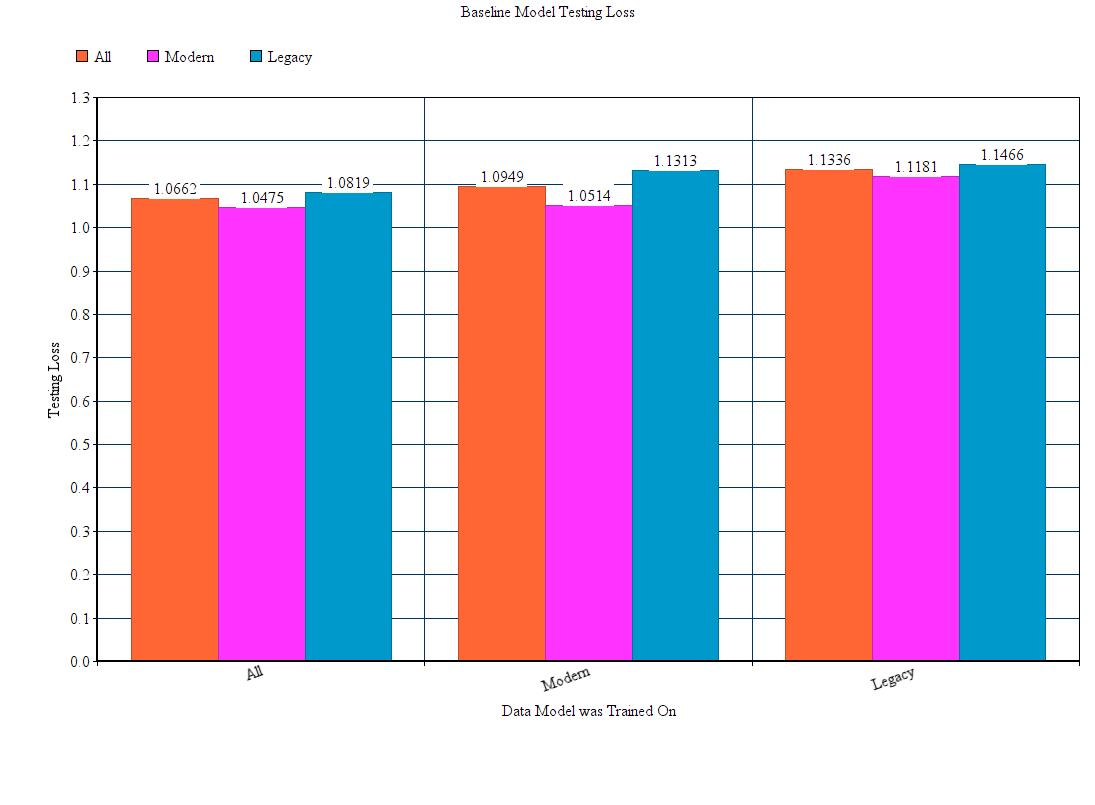
\includegraphics[width=.5\textwidth]{baseline-loss}
  \caption{Top: Prediction accuracy of the baseline. Bottom: Prediction loss of the baseline}
  \label{fig:baseline}
\end{figure}

This immediately confirmed our hypothesis that since Modern is the data set
with the most consistent art, the highest accuracy came from the model trained
on the Modern set evaluating the Modern testing set. It also follows that the
model trained on all cards would have more consistent across all
testing conditions. It was more unexpected that the model trained on Legacy
data performed best on the Modern testing data and worst on Legacy data. Poor
performance in general combined with this observation suggests that the art
within the Legacy set is more varied than we had anticipated.
We then wanted to run experiments with the goal of improving accuracy. Due to
the large size of these datasets and the time it takes to train a model, we
could not afford to train them experimentally. We created a development dataset
consisting of 700 cards from the Modern dataset, since it seemed to be our best
dataset for achieving good performance. Our hypothesis was that improving results
for this dataset would improve results when the full models were trained. The
performance for this baseline can be found in Figure ~\ref{fig:best} when it is being compared
to the performance of the best configuration we found.
During the experiments we noticed training behavior exhibited in Figure ~\ref{fig:overfitting}

\begin{figure}[h!]
  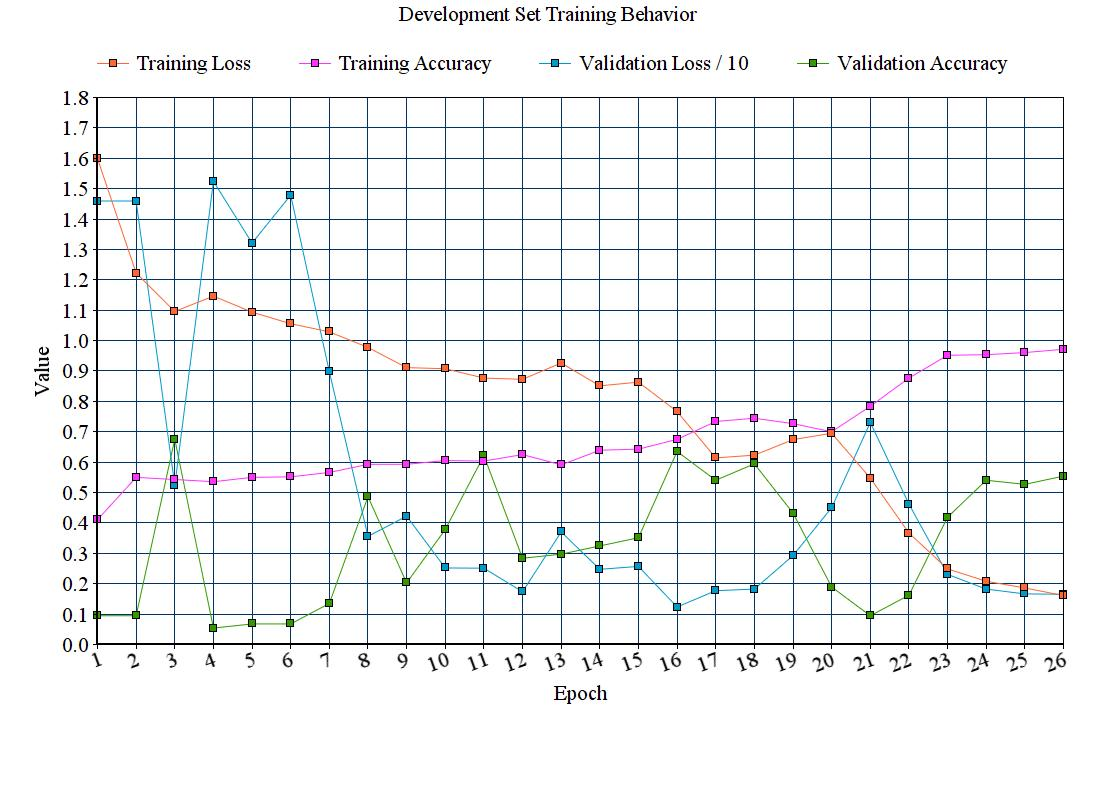
\includegraphics[width=.5\textwidth]{overfitting}
  \caption{Curves showing how the model went into overfitting after epoch 16}
  \label{fig:overfitting}
\end{figure}

Between epochs 16 and 21 training loss and validation accuracy plummet while
training accuracy improves and validation loss spikes before recovering. We
interpreted this as overfitting behavior and realized that we were wasting
training time during overfitting epochs because they would not improve the
validation loss. To combat this, we introduced a learning rate reduction
callback which decreased the learning rate if the validation loss does not
improve over a certain number of epochs. After some testing, we realized the
ideal configuration for this was to reduce learning rate by a factor of 10 each
time 5 epochs passed with no improvement, down to a minimum learning rate of
1e-5. We begin the learning rate at 1e-3.
After introducing this to our trials, we noticed marked improvement for our
development set. The best configuration we found was: 30 epochs, learning rate
reduction, SGD optimizer (1e-6 decay, .7 momentum), early stopping after 10
epochs, and image size 300x240. The results of these setting compared
to the baseline can be seen in Figure ~\ref{fig:best}

\begin{figure}
  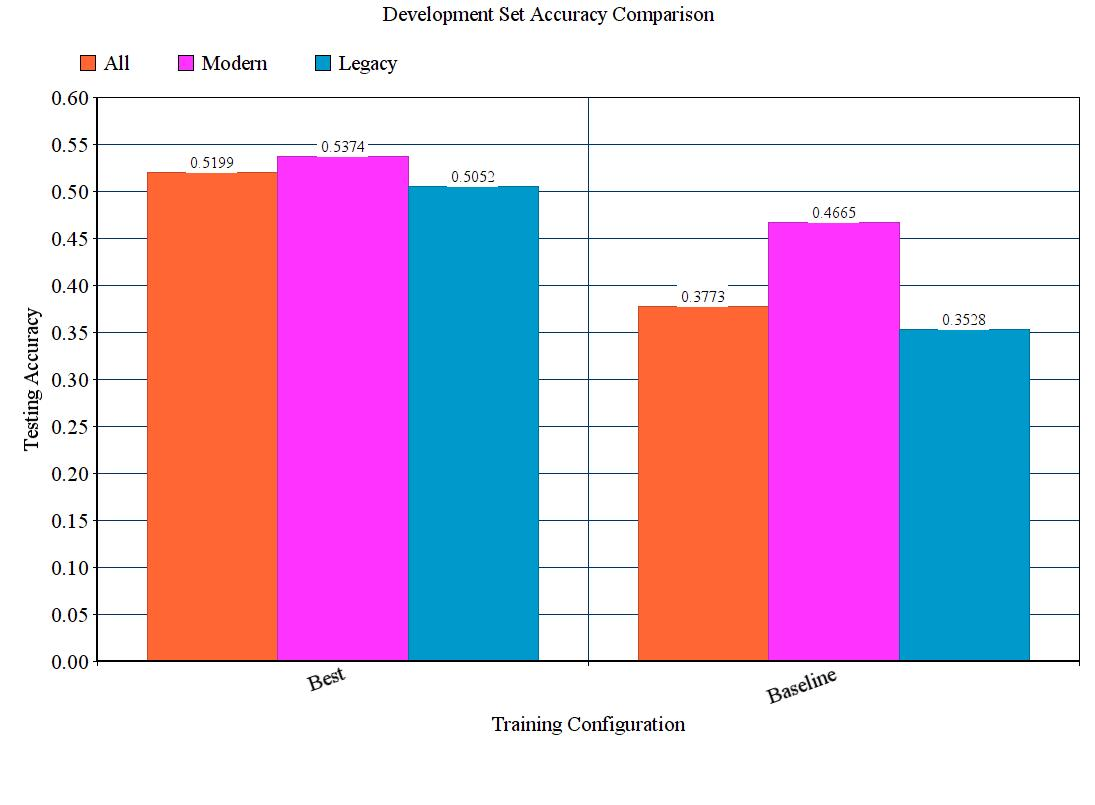
\includegraphics[width=.5\textwidth]{best-accuracy}
  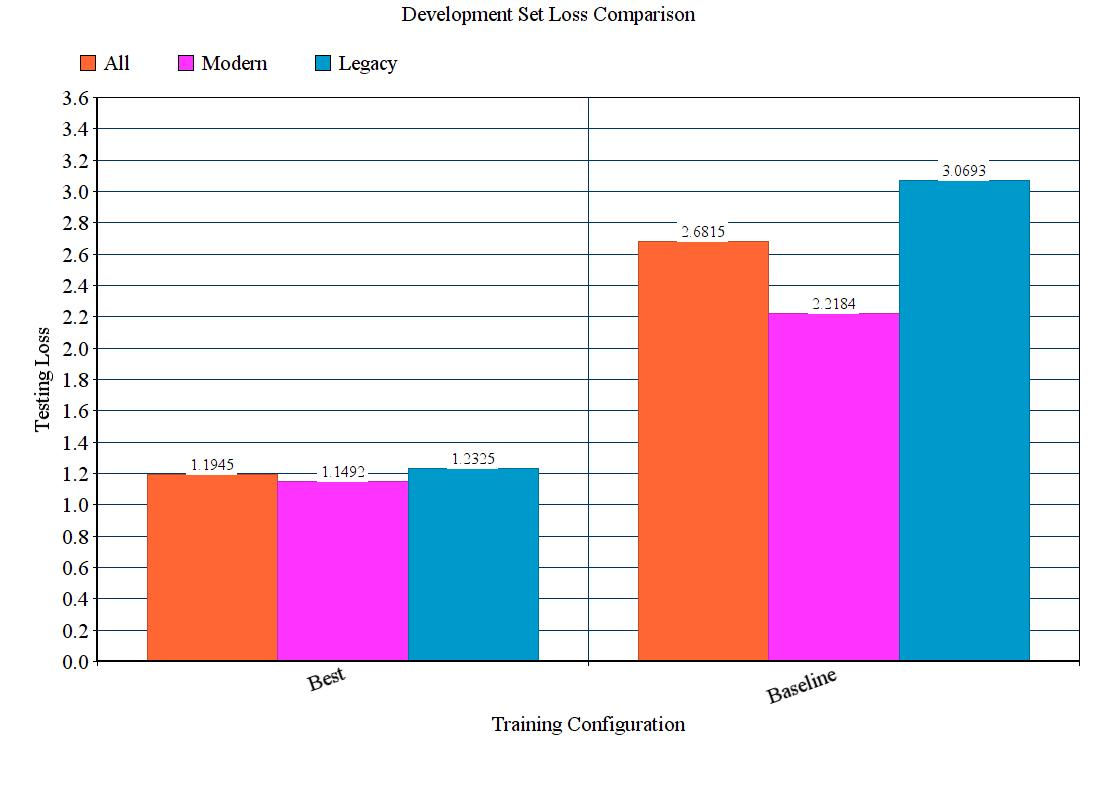
\includegraphics[width=.5\textwidth]{best-loss}
  \caption{Comparisons of the optimal performance to the baseline with accuracy on top and loss on the bottom.}
  \label{fig:best}
\end{figure}

We used these settings on the full data sets and got the following results in Figure ~\ref{fig:bestoverall}

\begin{figure}
  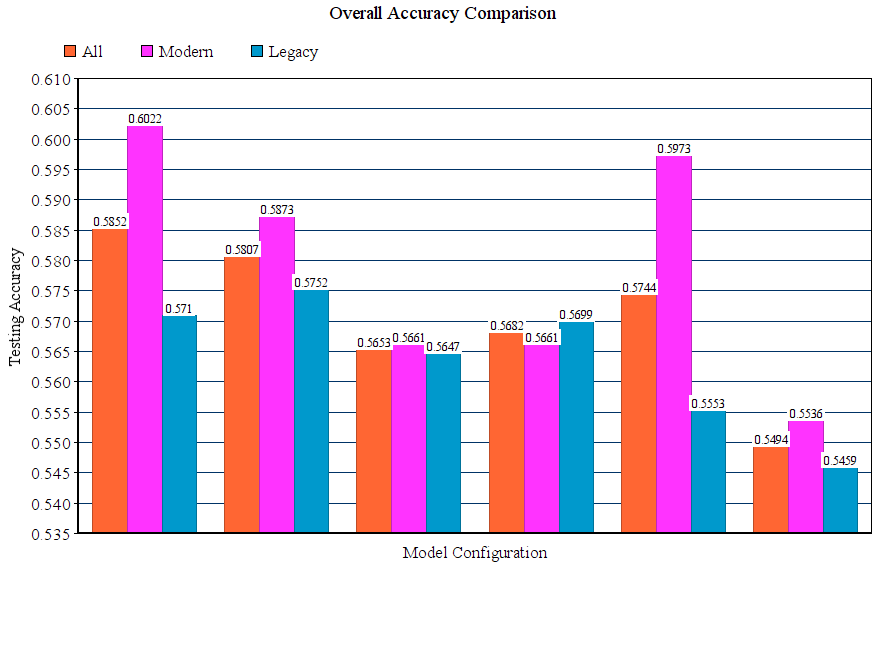
\includegraphics[width=.5\textwidth]{best-overall}
  \caption{The three groupings on the left represent models trained using the best configuration.
  The three on the right are using the baseline configuration. For both groupings the lines represent
  models trained all All data, Modern data, and Legacy data, in that order. There is improvement
  for every test category for every model except for the model trained on Modern data and applied to Modern data.}
  \label{fig:bestoverall}
\end{figure}

Unfortunately, the optimizations made during the experiments did not translate
into significant improvement for the full-scale models. Although we had similar
loss values and on average slightly better accuracies, this could be due to
noise during the training of the model and so we cannot claim that these changes
affected the performance of the model.

\section{Conclusion}

Due to the poor performance of our model in terms of classifying images, we
conclude that DenseNet-121 is not a sufficient architecture for classifying
Magic card type by card art. After running several experiments to increase
performance on experimental sets of data, we did not find a proportional
increase in performance when these methods were transferred over to the full
data sets. If we had more time and computing resources, we might have tried
another architecture such as InceptionV3 to compare which would have given us
a better idea about wider capabilities of neural networks regarding the
classification of magic cards by card art. It could be possible that the art of
Magic cards is so complex and varied that it is a difficult task for any neural
network, but this would require the evaluation of several more architectures to
be proven. Either way, we determined that our text-based classifier for names
was better suited for this task than our image classifier.


\bibliography{doc}
\bibliographystyle{aaai}

\end{document}


%%% Local Variables:
%%% mode: latex
%%% TeX-master: t
%%% End:
